\documentclass[10pt,letterpaper]{IEEEtran}

\usepackage{graphicx}
\usepackage{booktabs}
\usepackage{array}
\usepackage{amsmath}
\usepackage{caption}
\usepackage{url}
\usepackage[hidelinks]{hyperref}

\captionsetup{font=small}

\begin{document}

\title{RadarScenes Object Classification:\\From Single Scan to Multi-Scan Tracks}

\author{Bruno Pinto}

\maketitle

\begin{abstract}
A single RadarScenes detection instance (one object, one scan) averages only
$\sim$2.9 points. A DeepReflecs point-set classifier trained on single scans
(all 4 sensors) scored 0.7370 macro F1 across five target classes (\emph{car},
\emph{large\_vehicle}, \emph{two\_wheeler}, \emph{pedestrian},
\emph{pedestrian\_group}), a sparsity ceiling, not a model capacity one. That
motivates accumulating a tracked object's points across its last $N$ radar
scans instead of classifying each scan in isolation. A naive pooled baseline
(DeepReflecs, $N=20$ scans, all sensors, no notion of scan order) already
reaches 0.8613 macro F1 purely from extra points. The best result (0.8897
macro F1) comes from a causal GRU that consumes the sequence of per-scan
embeddings directly (order-aware, one hidden state per track); fusing it with
the order-blind pooled embedding through a small trained classifier head adds
only $+0.0002$, within this project's own single-split noise band, not a
reliable additional gain. The fusion model's confusion matrix shows two
dominant error axes: 15\% of \emph{large\_vehicle} tracks are misclassified
as \emph{car} (the reverse barely happens, 3.8\%), and
\emph{pedestrian}/\emph{pedestrian\_group} confuse each other in both
directions (6.6\% and 8.6\%).
\end{abstract}

\begin{IEEEkeywords}
automotive radar, point cloud, object classification, RadarScenes, GRU, sequence modeling
\end{IEEEkeywords}

\begin{figure*}[t]
  \centering
  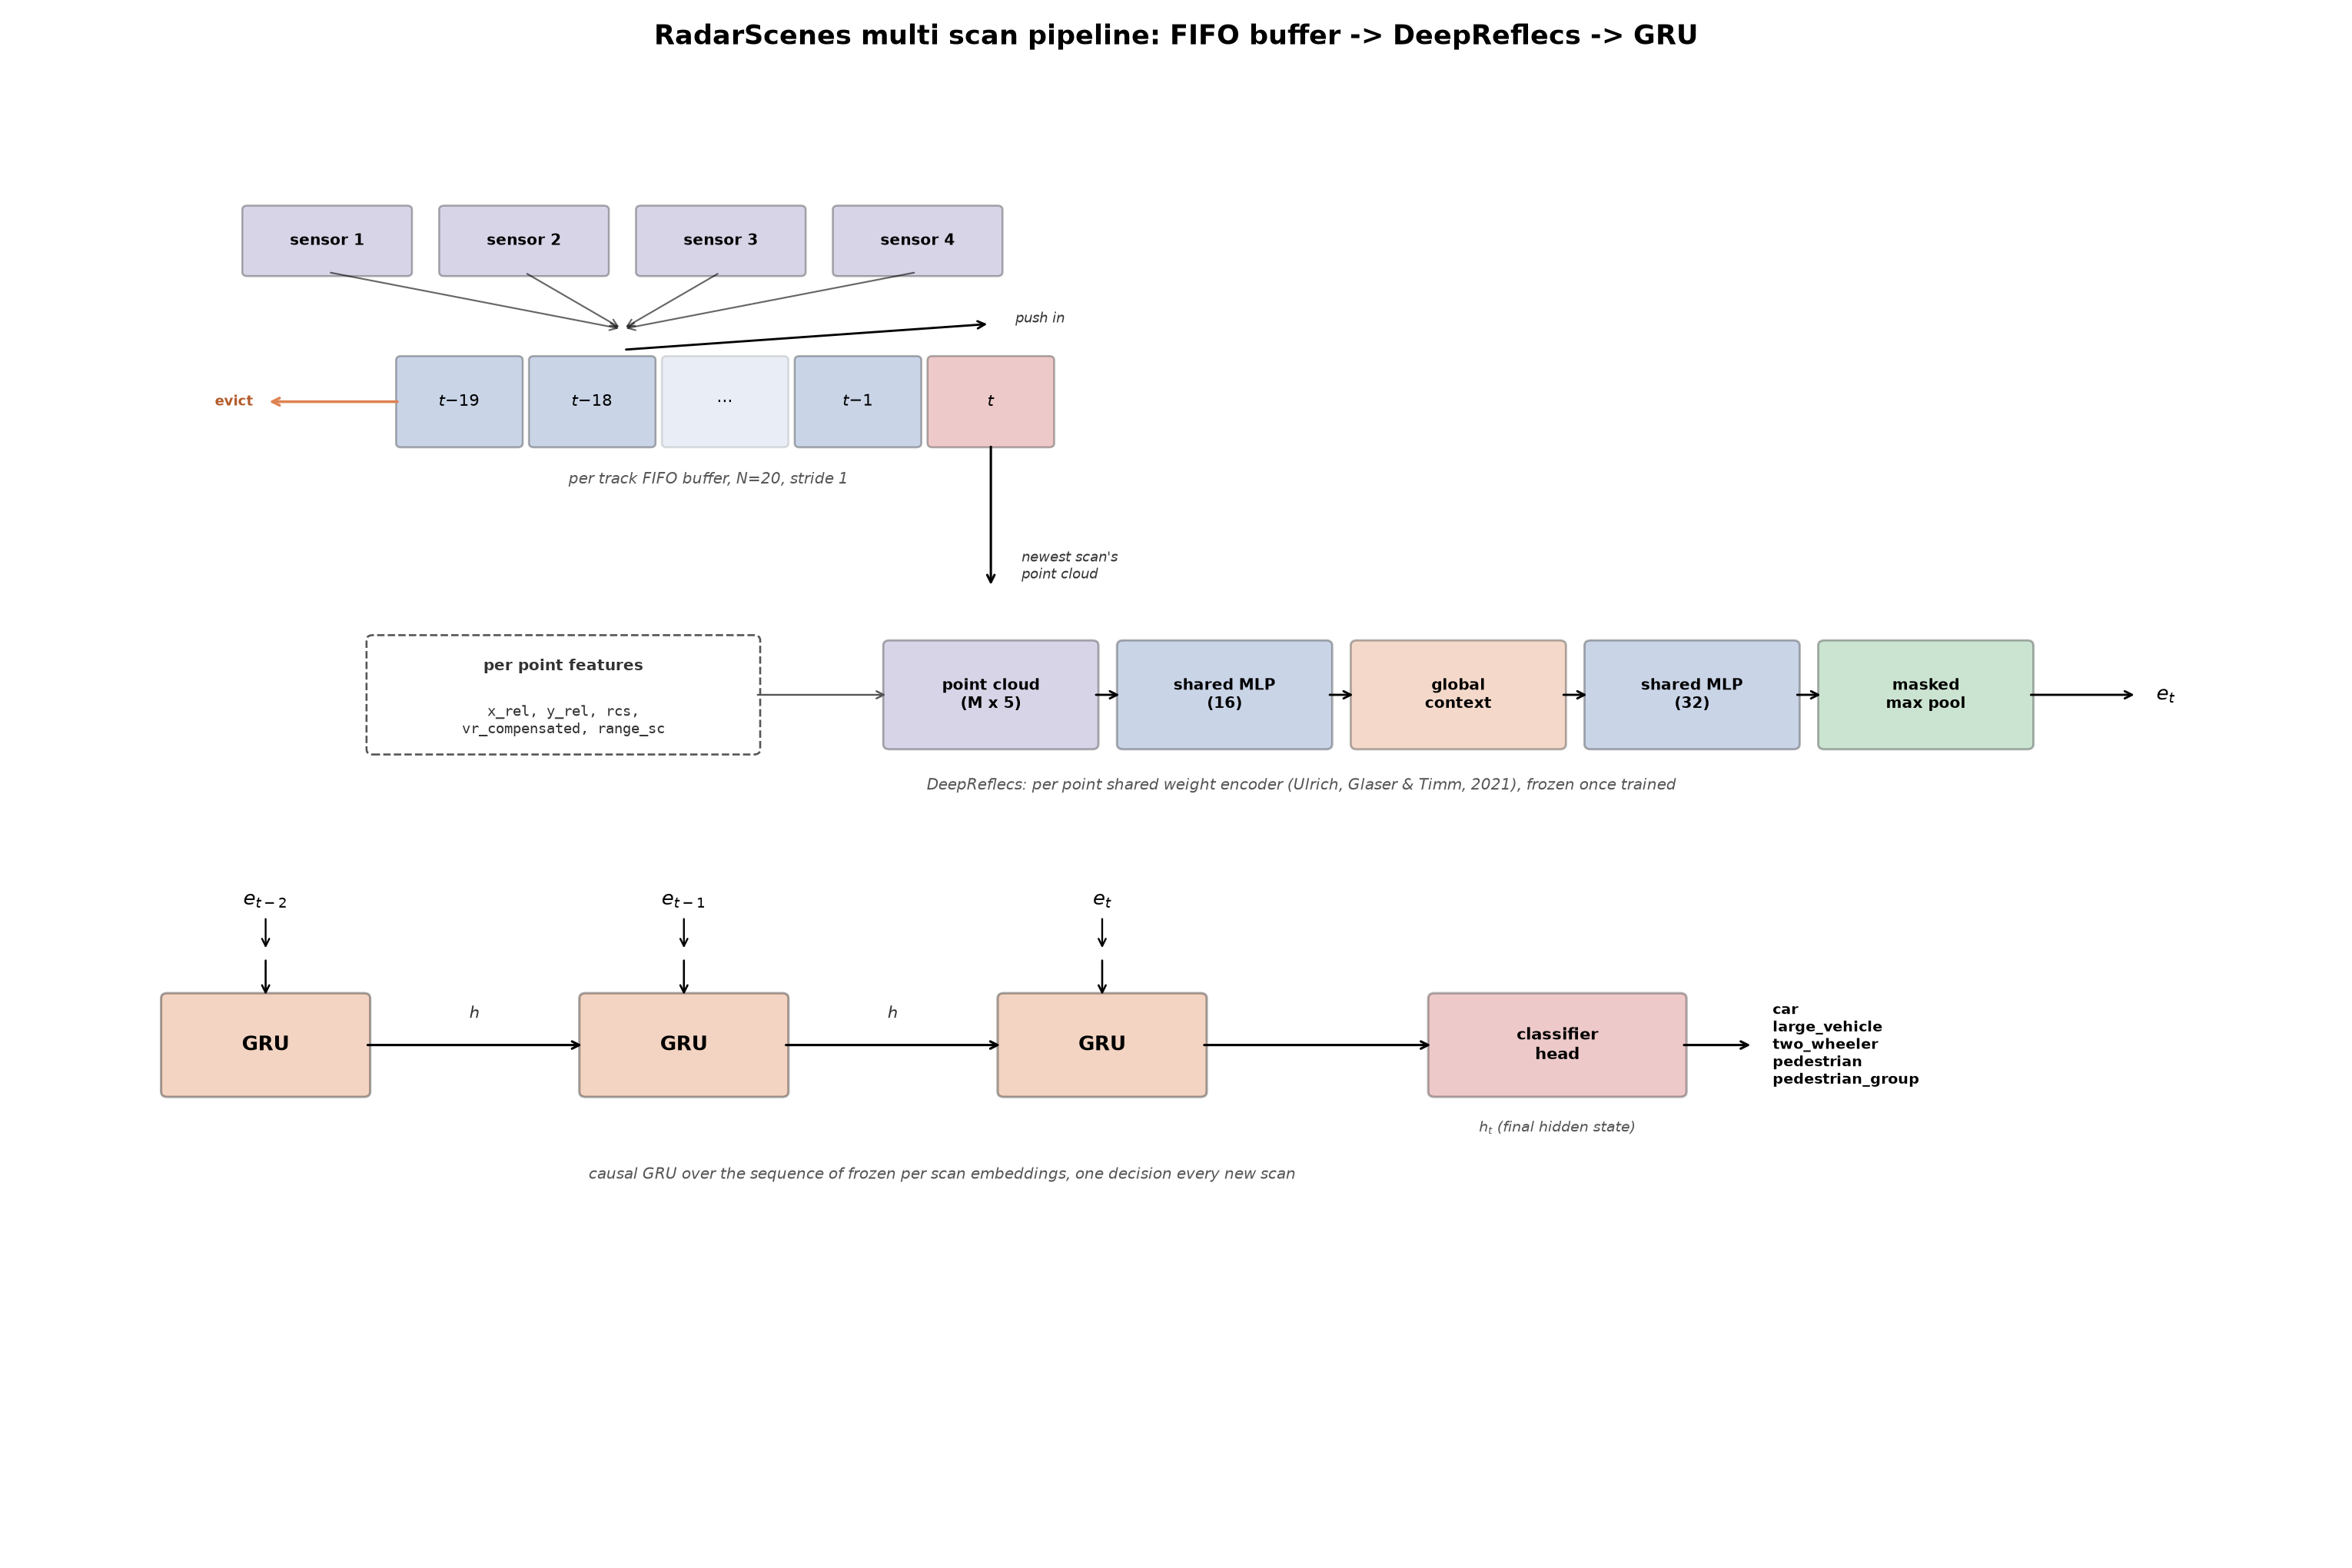
\includegraphics[width=0.82\textwidth]{pipeline_overview.png}
  \caption{Multi-scan pipeline: per-track FIFO buffer feeding a frozen DeepReflecs encoder, whose per-scan embeddings drive a causal GRU.}
  \label{fig:pipeline}
\end{figure*}

\section{The RadarScenes Dataset}

RadarScenes \cite{schumann2021radarscenes} is a real-world automotive radar
dataset: 4 series-production radar sensors mounted on a test vehicle,
overlapping fields of view (Fig.~\ref{fig:sensors}), point-level semantic
labels propagated from camera-verified object tracks.

This project's taxonomy merges RadarScenes' own finer-grained labels into 5
classes (\emph{car}, \emph{large\_vehicle}, \emph{two\_wheeler},
\emph{pedestrian}, \emph{pedestrian\_group}); \emph{large\_vehicle} folds in
\emph{truck}/\emph{train}/\emph{bus} (near-chance pairwise separability from
\emph{car}-sized vehicles at the raw-class level, and \emph{train}/\emph{bus}
individually too thin to split without leakage). All 4 sensors share one
global clock.

\begin{figure}[t]
  \centering
  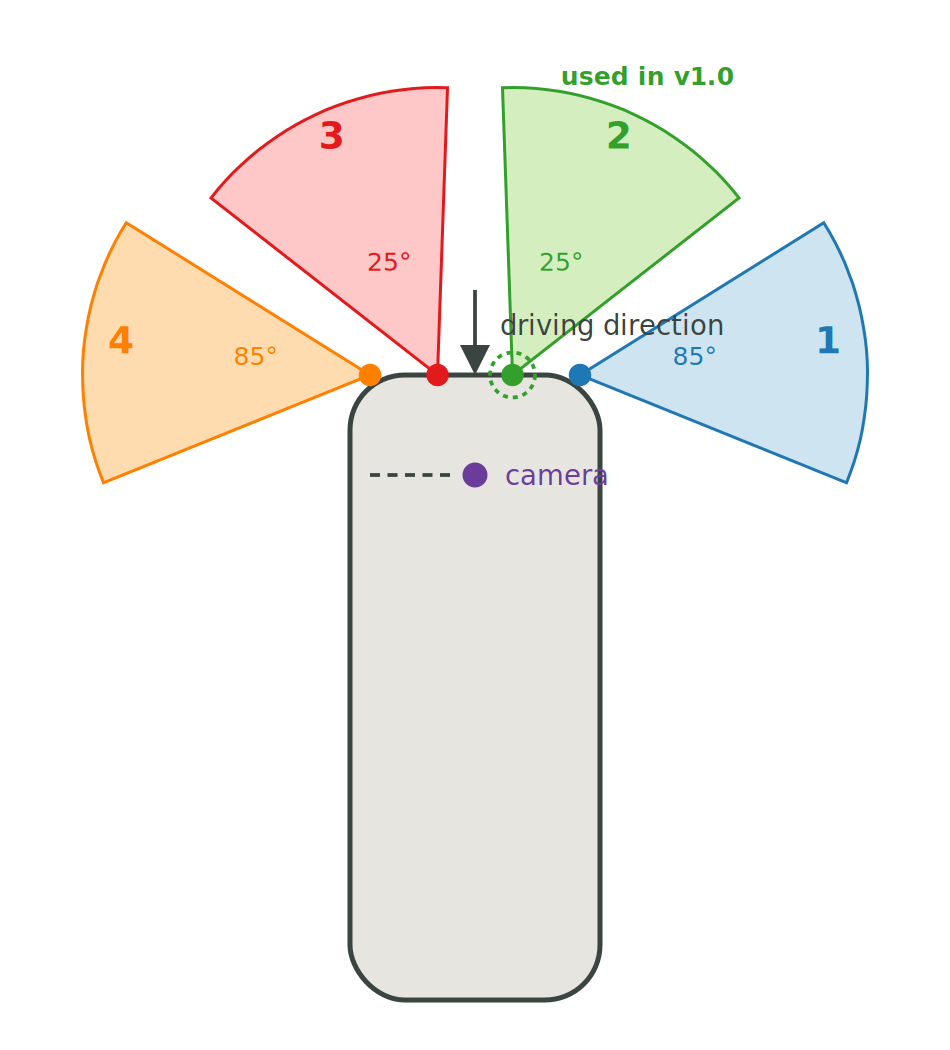
\includegraphics[width=0.75\columnwidth]{results/radarscenes_sensor_layout.png}
  \caption{RadarScenes sensor layout, sensor 2 highlighted.}
  \label{fig:sensors}
\end{figure}

\section{Single-Scan Baseline: DeepReflecs}

DeepReflecs \cite{ulrich2021deepreflecs} is a per-point shared-weight network
(PointNet-style): the same small MLP processes every point independently, so
the model is order-invariant and works on a variable number of points by
construction. This project adapts its input features to what RadarScenes
provides ($x_{rel}$, $y_{rel}$, $rcs$, $vr_{compensated}$, $range_{sc}$), not
a literal reproduction of the paper's own feature set.

What sets it apart from a plain PointNet baseline is that the \emph{global
context layer} sits \emph{between} the two per-point stages, not only at the
very end, so the second per-point layer already has access to a
permutation-invariant summary (mean/max) of the whole point set before
producing its own output. A \emph{masked global max-pool} then reduces the
(variable-length) point set to one fixed embedding, invariant to how many
padding points get added, picking out the most salient reading per channel
regardless of point count (Fig.~\ref{fig:deepreflecs}).

\begin{figure*}[t]
  \centering
  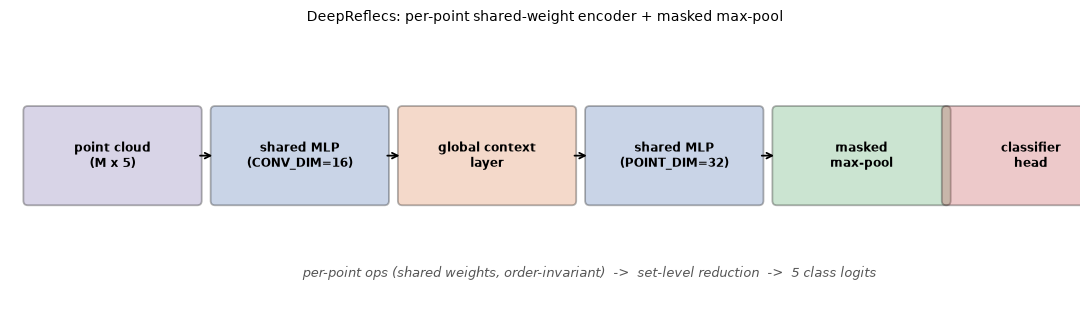
\includegraphics[width=0.85\textwidth]{results/final_report/final_report_6_0.png}
  \caption{DeepReflecs: two per-point shared-weight MLP stages with a global context layer between them, followed by a masked max-pool and classifier head.}
  \label{fig:deepreflecs}
\end{figure*}

\begin{table}[t]
  \centering
  \caption{Single-Scan ($N=1$, All Sensors) Test Metrics}
  \label{tab:n1}
  \begin{tabular}{lrrrr}
    \toprule
    Class & Precision & Recall & F1 & Support \\
    \midrule
    car               & 0.942 & 0.816 & 0.874 & 76{,}572 \\
    large\_vehicle    & 0.676 & 0.782 & 0.725 & 15{,}555 \\
    two\_wheeler      & 0.522 & 0.777 & 0.625 & 11{,}466 \\
    pedestrian        & 0.664 & 0.884 & 0.758 & 35{,}091 \\
    pedestrian\_group & 0.810 & 0.621 & 0.703 & 40{,}081 \\
    \midrule
    \multicolumn{4}{l}{\textbf{Macro F1}} & \textbf{0.7370} \\
    \bottomrule
  \end{tabular}
\end{table}

\textbf{Single-scan baseline: macro F1 = 0.7370} (Table~\ref{tab:n1}).
\emph{car} is the strongest class (F1 0.874, most points per instance, most
rigid/consistent signature); \emph{two\_wheeler} is the weakest (F1 0.625,
sparsest class, easily confused with \emph{car}/\emph{pedestrian} at this
point-count regime). This is the floor every multi-scan result below
improves on (Fig.~\ref{fig:cm-n1}).

\begin{figure}[t]
  \centering
  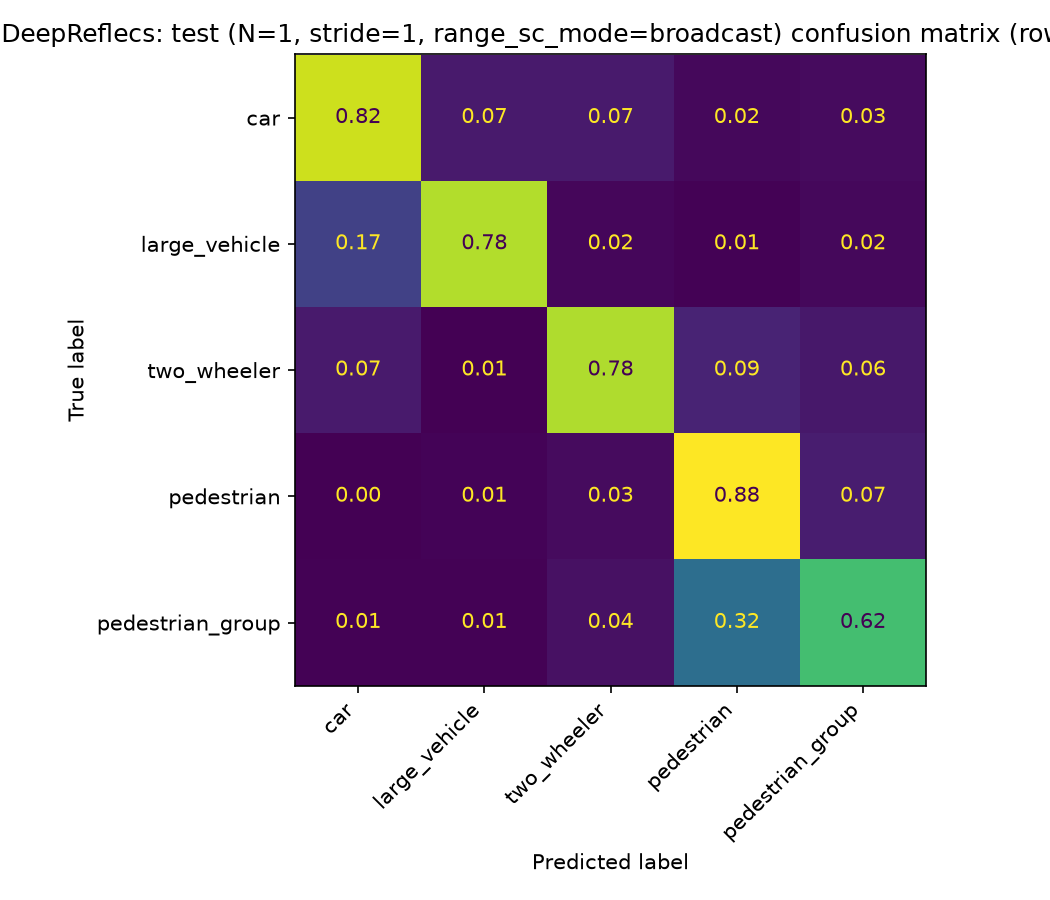
\includegraphics[width=0.85\columnwidth]{results/final_report/final_report_8_1.png}
  \caption{Single-scan ($N=1$, all sensors) confusion matrix, row-normalized.}
  \label{fig:cm-n1}
\end{figure}

\section{Motivation: Why Accumulate Scans}

\begin{itemize}
\item A single detection instance averaging $\sim$2.9 points hits a hard
  ceiling regardless of encoder: histograms, explicit per-instance statistics
  (median, max, min, spread), and DeepReflecs' learned point-set network all
  converge to a similar macro F1 band on single-scan data (Section~II). The
  bottleneck is point count, not model choice.
\item Beyond raw point count, a tracked object's radar signature evolves scan
  to scan: a pedestrian's micro-Doppler shifts as limbs swing, and RCS
  fluctuates as an object's dominant reflectors change with aspect angle.
  None of that is visible in a single scan, motivating a sequence model over
  the per-scan embeddings (Section~V) in addition to simply pooling more
  points.
\item A \texttt{track\_id} persists across a tracked object's lifetime,
  multiple radar scans of the \emph{same} object, and all 4 sensors share one
  global clock. Pooling a track's last $N$ scans' points into one decision,
  instead of one scan's points, attacks sparsity directly at the input level
  rather than trying to encode more out of the same few points.
\item A second, independent factor: building a window from whichever
  sensor(s) are actually detecting the track \emph{right now}
  (cross-sensor handoff) gets more real detections per track without needing
  more real time to pass, since a track is often seen by 2--3 different
  sensors as it moves through overlapping fields of view.
\item Coordinate frame: the car frame ($x_{cc}$/$y_{cc}$) rotates with ego
  heading and is unusable across scans; the global odometry-corrected frame
  ($x_{seq}$/$y_{seq}$), recentered per scan on that scan's own object
  centroid ($x_{rel}$/$y_{rel}$ = $x_{seq}$/$y_{seq}$ minus that scan's own
  mean), is what actually goes into the model, bounded scan-to-scan instead of
  drifting with the object's accumulated path.
\end{itemize}

\section{Multi-Scan Baseline: Naive Pooling}

All points from a track's last $N=20$ scans (all sensors) are concatenated
into \emph{one} point set, classified by a single DeepReflecs instance
trained end-to-end on the pooled data. No sequence model, no per-scan
structure retained, no notion of which point came from which scan at all.

In deployment this window is a per-track FIFO buffer: each new scan pushes in
and the oldest one drops out, so the buffer always holds exactly the last $N$
scans and a decision fires the moment a new scan arrives
(Fig.~\ref{fig:fifo}).

\begin{figure*}[t]
  \centering
  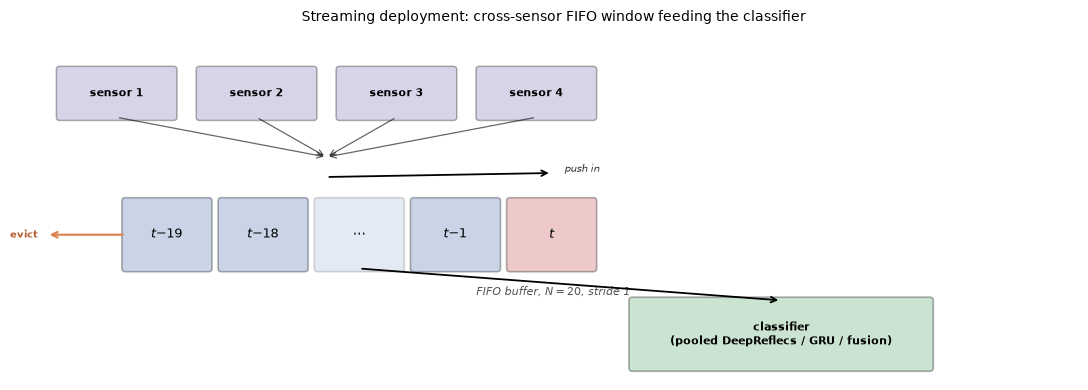
\includegraphics[width=0.85\textwidth]{results/final_report/final_report_13_0.png}
  \caption{Streaming deployment: the cross-sensor FIFO window feeding the classifier.}
  \label{fig:fifo}
\end{figure*}

\subsection{Baseline Result}

\begin{table}[t]
  \centering
  \caption{Pooled ($N=20$, All Sensors) Test Metrics}
  \label{tab:n20}
  \begin{tabular}{lrrrr}
    \toprule
    Class & Precision & Recall & F1 & Support \\
    \midrule
    car               & 0.953 & 0.909 & 0.930 & 76{,}572 \\
    large\_vehicle    & 0.798 & 0.832 & 0.815 & 15{,}555 \\
    two\_wheeler      & 0.744 & 0.884 & 0.808 & 11{,}466 \\
    pedestrian        & 0.867 & 0.919 & 0.892 & 35{,}091 \\
    pedestrian\_group & 0.877 & 0.846 & 0.861 & 40{,}081 \\
    \midrule
    \multicolumn{4}{l}{\textbf{Macro F1}} & \textbf{0.8613} \\
    \bottomrule
  \end{tabular}
\end{table}

\textbf{Baseline: macro F1 = 0.8613} (Table~\ref{tab:n20}), +0.1243 over the
single-scan floor from pooling alone, no new architecture. Weakest class is
still \emph{two\_wheeler} (F1 0.808), but every class improved substantially
over Section~II's single-scan numbers (Fig.~\ref{fig:cm-n20}).

\begin{figure}[t]
  \centering
  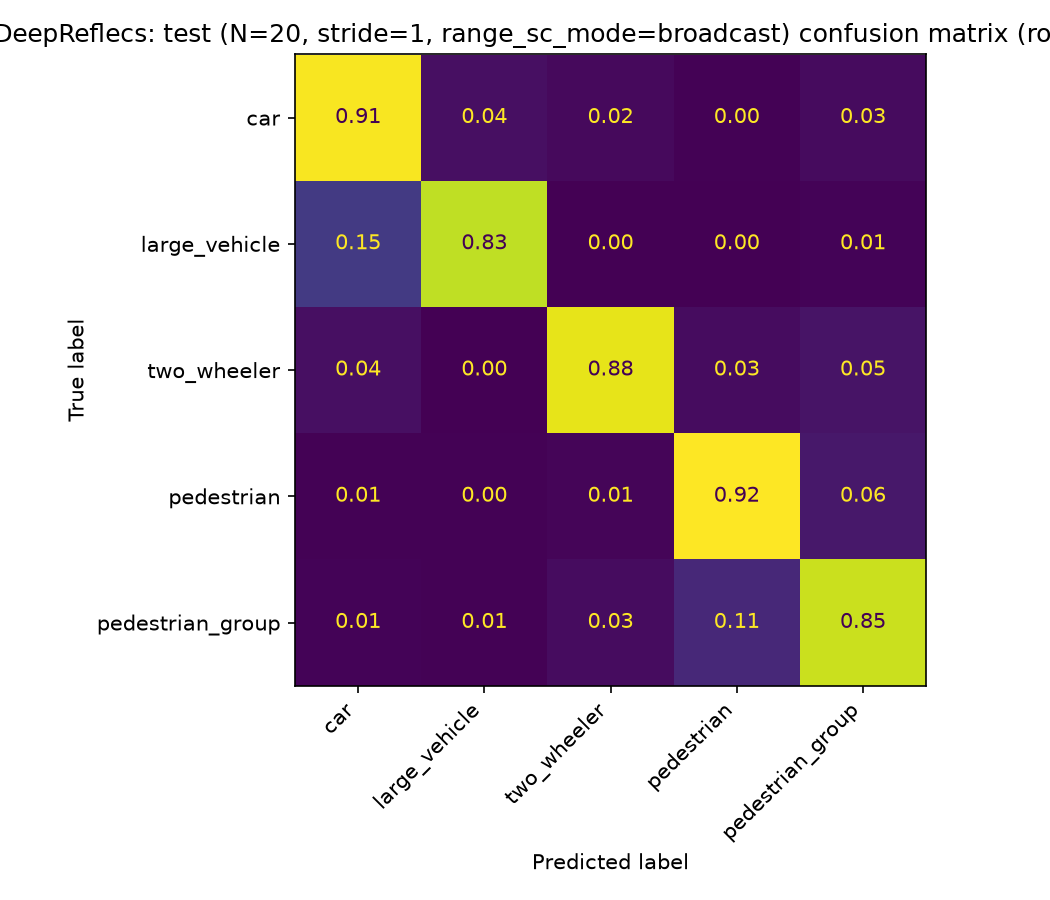
\includegraphics[width=0.85\columnwidth]{results/final_report/final_report_15_1.png}
  \caption{Multi-scan pooled baseline ($N=20$, all sensors) confusion matrix, row-normalized.}
  \label{fig:cm-n20}
\end{figure}

Why pooling helps even on a near-static track: at $\sim$2.9 points per scan,
which scatterers cross the CFAR threshold is dominated by speckle (coherent
fading), not just the object's geometry, so consecutive scans give largely
independent noisy draws of the same object rather than redundant copies.
Pooling $N$ of them is variance reduction on the detection process (more
points per class-defining statistic), plus some aspect-angle
diversity from ego/relative motion; this report cannot cleanly separate how
much each contributes.

One specific confusion drops a lot: \emph{two\_wheeler} misclassified as
\emph{pedestrian} falls from 8\% (single scan) to 3\% (pooled $N=20$),
consistent with pooling resolving the two classes' overlapping
point-count/RCS regime rather than just raising \emph{two\_wheeler}'s overall
recall uniformly.

\subsection{The two\_wheeler $\to$ pedestrian Confusion}

\begin{table}[t]
  \centering
  \caption{Window Statistics: two\_wheeler $\to$ pedestrian (3\%)}
  \label{tab:tw-ped}
  \footnotesize
  \begin{tabular}{lrrr}
    \toprule
    Metric (median) & Confused & Correct tw & True ped \\
    \midrule
    $n$ windows                  & 345    & 10{,}136 & 35{,}091 \\
    Points/window                & 25.0   & 51.0     & 33.0     \\
    Diagonal length               & 1.058  & 1.776    & 0.742    \\
    RCS mean                     & $-$7.509 & $-$11.033 & $-$8.523 \\
    Doppler spread                & 0.344  & 0.521    & 0.408    \\
    $vr_{compensated}$ mean       & $-$0.141 & 2.087   & 0.408    \\
    RCS temporal variation        & 94.713 & 117.641  & 88.578   \\
    $vr$ temporal variation       & 3.637  & 6.298    & 4.508    \\
    \bottomrule
  \end{tabular}
\end{table}

\textbf{Why the remaining 3\%} (Table~\ref{tab:tw-ped}). The 345 confused
windows are \emph{two\_wheeler}'s sparse, slow tail: half the points of a
correctly classified \emph{two\_wheeler} window, a spatial extent shrunk
toward \emph{pedestrian}'s, and a velocity of $-$0.14~m/s median (a correctly
classified \emph{two\_wheeler} moves at +2.09~m/s) indistinguishable from a
walking pedestrian's +0.41~m/s.

Scan-to-scan dynamics (median per scan, diffed consecutively, normalized by
real elapsed time) confirm this is not just a snapshot effect: $vr$ temporal
variation is 3.64 for confused windows vs.\ 4.51 for true pedestrian and 6.30
for correct \emph{two\_wheeler}, confused is still the quietest group
scan-to-scan, not just at a single instant. RCS temporal variation is 94.7
for confused, close to true pedestrian's 88.6 and well below correct
\emph{two\_wheeler}'s 117.6. The floor holds on both axes once measured
correctly: this reads as a stationary or near-stationary
bike/rider, not just a snapshot that happens to look slow.\footnote{An earlier pass at this computed ``dynamics'' as a
point-to-point diff across the raw pooled point array, which mixes
within-scan spatial variation with across-scan temporal change and is
confounded by point count. The velocity conclusion above happens to survive
that error; the \emph{large\_vehicle}/\emph{car} case in
Section~IV-C does not.}

\subsection{The large\_vehicle $\to$ car Confusion}

\begin{table}[t]
  \centering
  \caption{Window Statistics: large\_vehicle $\to$ car (15\%)}
  \label{tab:lv-car}
  \footnotesize
  \begin{tabular}{lrrr}
    \toprule
    Metric (median) & Confused & Correct lv & True car \\
    \midrule
    $n$ windows             & 2{,}411 & 12{,}943 & 76{,}572 \\
    Points/window           & 38.0    & 164.0    & 48.0     \\
    Diagonal length          & 3.280   & 13.650   & 4.289    \\
    RCS mean                & 2.332   & 2.502    & $-$0.554 \\
    Doppler spread           & 0.285   & 2.539    & 1.489    \\
    Range                   & 36.189  & 26.880   & 34.763   \\
    RCS temporal variation   & 172.058 & 128.530  & 145.945  \\
    $vr$ temporal variation  & 1.855   & 1.025    & 4.077    \\
    \bottomrule
  \end{tabular}
\end{table}

\textbf{Why large\_vehicle confuses with car} (Table~\ref{tab:lv-car}). The
2411 confused windows have a quarter the points of a correctly classified
\emph{large\_vehicle}, and a spatial extent \emph{smaller} than a typical
car's (diagonal 3.3 vs.\ car's 4.3, vs.\ 13.7 for a correctly classified
\emph{large\_vehicle}), at longer range (36.2~m vs.\ 26.9~m correct, vs.\
34.8~m car). At longer range, fewer of a long vehicle's physically separated
reflectors resolve into distinct detections, collapsing it toward a compact,
car-sized point cloud regardless of its real length -- the same
range/resolution effect.

Scan-to-scan dynamics, computed correctly, do not tell a clean ``converges
toward car'' story the way extent and point count do. $vr$ temporal variation
for confused windows (1.85) sits between correct \emph{large\_vehicle}'s low
1.03 and true car's much higher 4.08, closer to \emph{large\_vehicle}'s own
quiet end than to car's. RCS temporal variation for confused windows (172.1)
is actually the \emph{highest} of the three groups, above both correct
\emph{large\_vehicle} (128.5) and true car (145.9). This is unresolved, no
explanation found: confused windows keep \emph{large\_vehicle}-like low
velocity dynamics while showing unusually elevated RCS variation, neither
converging toward car nor staying flat like \emph{large\_vehicle}.\footnote{This
specific statistic went through three computation methods before landing
here -- a raw per-window sum confounded by point count, then a point-to-point
diff mixing within-scan and across-scan variation, both of which showed
confused windows as uniformly ``quieter than car.'' Neither survives the
correct scan-median, elapsed-time-normalized computation above.}

RCS mean (the level, not the scan-to-scan variation above) looked like a
surviving cue at the median (2.33 confused vs.\ 2.50 correct
\emph{large\_vehicle} vs.\ $-$0.55 car), but a median gap can look clean while
the underlying distributions still overlap heavily.

\begin{table}[t]
  \centering
  \caption{Single-Feature Separability: Confused large\_vehicle vs.\ True car}
  \label{tab:auc-rcs}
  \begin{tabular}{lrr}
    \toprule
    Feature & AUC & \% inside car's 10--90th pct \\
    \midrule
    RCS mean          & 0.624 & 88\% \\
    Doppler spread    & 0.651 & 87\% \\
    \bottomrule
  \end{tabular}
\end{table}

Pulling the actual distributions settles it (Table~\ref{tab:auc-rcs}): RCS
mean separates confused \emph{large\_vehicle} from true car with AUC 0.624,
and Doppler spread with AUC 0.651 (0.5 is chance, 1.0 is perfect), with 88\%
and 87\% of confused windows respectively falling inside true car's own
10th--90th percentile range. There is also an architecture reason this is
moot regardless: DeepReflecs never computes ``mean RCS of the window'' as a
feature, it takes a max-pool over a learned per-point transform, so even a
genuinely separable signal in the mean or lower tail could be invisible to
whatever extreme value max-pooling happens to grab. Both cues are far weaker
than the median comparison suggested, and overlap too heavily with car's own
distribution to count as a reliable, usable signal. RCS was never as
separable here as the summary statistic made it look; extent and point count
(Table~\ref{tab:lv-car}) remain the only cues shown above to separate the
groups cleanly.

\subsection{Tracker-Feature Check}

Eight scan-to-scan dynamics features were checked against both confusions,
inspired by Aptiv's US~12{,}013{,}919~B2 \cite{aptiv2024patent}, which fuses a
point-set branch with a separate tracker-feature branch (variance of
velocity, variance of heading direction, absolute curvature, among others)
before a GRU. Each feature is defined as:

\begin{itemize}
\item \textbf{heading variance}: $1-R$ where $R=\sqrt{\langle\cos\theta\rangle^2+\langle\sin\theta\rangle^2}$ over the window's per-scan centroid headings (circular variance, handles wraparound).
\item \textbf{curvature}: mean of $|\Delta\theta|/\text{step distance}$ between consecutive scans.
\item \textbf{RCS / velocity variance}: variance of each scan's own median RCS / $vr_{compensated}$ across the window (spread of the raw level, not a diff).
\item \textbf{RCS / velocity oscillation}: variance of the \emph{signed} scan-to-scan diffs of those same per-scan medians, high if the value swings up and down even when the net change is zero.
\item \textbf{RCS / velocity drift}: mean of the same signed diffs, the net directional trend over the window.
\end{itemize}

Heading/curvature use each scan's centroid position; there is no real Kalman
tracker state in this pipeline to pull a smoothed heading from, so this is a
cheap proxy, not the patent's actual tracker-filtered feature.

\begin{table*}[t]
  \centering
  \caption{Tracker-Feature Separability, Both Confusions (Medians and AUC)}
  \label{tab:tracker}
  \footnotesize
  \begin{tabular}{lrrrrrrrrrr}
    \toprule
    & \multicolumn{4}{c}{two\_wheeler $\to$ pedestrian} & & \multicolumn{4}{c}{large\_vehicle $\to$ car} \\
    \cmidrule{2-5} \cmidrule{7-10}
    Feature & Confused & True ped & AUC(ped) & AUC(tw) & & Confused & True car & AUC(car) & AUC(lv) \\
    \midrule
    heading variance        & 0.582  & 0.689  & 0.584 & 0.696 & & 0.860  & 0.791  & 0.604 & 0.604 \\
    curvature                & 6.700  & 10.497 & 0.743 & 0.606 & & 3.507  & 2.709  & 0.628 & \textbf{0.782} \\
    RCS variance             & 22.692 & 16.142 & 0.636 & 0.663 & & 26.292 & 26.449 & 0.507 & 0.702 \\
    velocity variance        & 0.097  & 0.068  & 0.531 & 0.509 & & 0.015  & 0.121  & 0.657 & 0.507 \\
    RCS oscillation           & 37.263 & 31.178 & 0.604 & 0.619 & & 59.289 & 54.923 & 0.520 & 0.674 \\
    velocity oscillation      & 0.064  & 0.100  & 0.587 & 0.578 & & 0.007  & 0.050  & 0.595 & 0.646 \\
    RCS drift                 & 0.027  & $-$0.000 & 0.529 & 0.533 & & 0.011  & $-$0.023 & 0.517 & 0.515 \\
    velocity drift             & $-$0.004 & 0.003 & 0.537 & 0.507 & & 0.002  & 0.004  & 0.532 & 0.505 \\
    \bottomrule
  \end{tabular}
\end{table*}

Drift carries no signal anywhere, every AUC is 0.50--0.54, noise floor. Every
feature that separates at all separates the confused group from its
\emph{own} correct class better than from the class it gets mistaken for
(curvature 0.782 vs.\ correct \emph{large\_vehicle} but only 0.628 vs.\ true
car; heading variance 0.696 vs.\ correct \emph{two\_wheeler} but only 0.584
vs.\ true pedestrian), the same asymmetry the RCS-mean check found: these
confused windows read as atypical for their own true class, not as typical
examples of the predicted class. No single feature clears $\sim$0.78;
curvature vs.\ correct \emph{large\_vehicle} is the strongest result in
Table~\ref{tab:tracker}.

Taken together with the RCS mean/Doppler spread check, none of these cues
clear the bar of a clean, usable signal on their own. This is the main
evidence against a temporal encoder branch for these two confusions
specifically: curvature is the one feature that shows a real, if moderate,
effect. Everything else looks like noise, or an AUC that's only non-trivial
because the comparison group itself happens to be a weak reference, not a
usable separating signal. This also undercuts Section~III's original
motivation for a sequence model (micro-Doppler and RCS dynamics evolving scan
to scan): that motivation still justifies a sequence model in principle, but
for these two specific confusions the scan-to-scan dynamics checked here
carry little to no signal, whatever the GRU/fusion gain over pooling is
coming from, it is not these engineered dynamics features.

Each feature above was tested in isolation; a classifier combining several weak
cues nonlinearly can still separate classes that no single cue separates
alone. A shallow gradient-boosted-tree classifier over all 8 features
together, 5-fold cross-validated, same two confusions, found real joint
separability the univariate check missed: AUC 0.78--0.92 depending on the
confusion, above the $\sim$0.78 ceiling any single feature reached alone.
Feature importance was concentrated, not spread evenly: velocity variance,
velocity oscillation, curvature, and RCS variance carried nearly all of it;
the drift features carried essentially none, consistent with their
0.50--0.54 AUC in Table~\ref{tab:tracker}. So the univariate check's ``no
usable temporal cue left'' conclusion holds feature by feature, but not for
the features combined, which motivated a learned architecture over the raw
tracker signal (Section~VII).

\section{Sequence Model: GRU, and Fusion with the Pooled View}

A frozen, already-trained DeepReflecs encoder reduces each scan to one
embedding vector; a GRU then consumes the sequence of a track's embeddings
causally (a prediction at scan $t$ only depends on scans up to and including
$t$, so it stays usable in real-time streaming inference). The encoder runs
once per scan across the whole dataset, not once per window, so a sliding
window's scan-to-scan overlap costs nothing extra in encoder compute
(Fig.~\ref{fig:gru}).

\begin{figure*}[t]
  \centering
  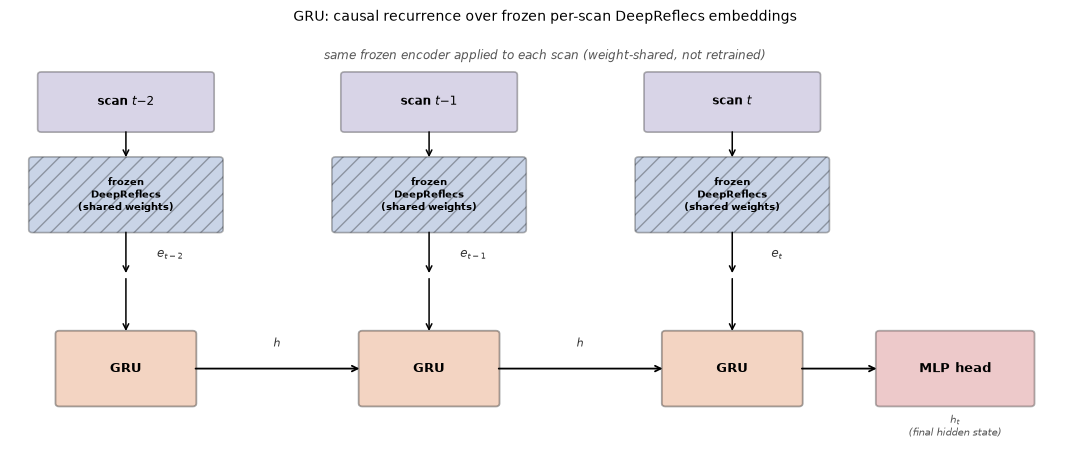
\includegraphics[width=0.85\textwidth]{results/final_report/final_report_27_0.png}
  \caption{GRU: causal recurrence over frozen per-scan DeepReflecs embeddings.}
  \label{fig:gru}
\end{figure*}

\textbf{Fusion} concatenates this GRU's final hidden state (order-aware) with
the pooled, order-blind embedding from Section~IV's baseline, then trains a
small classifier head on the concatenation, both branches frozen.
Structurally analogous to a U-Net skip connection \cite{ronneberger2015unet}:
splice in a view the deeper path's own bottleneck might otherwise discard,
instead of forcing one representation to carry everything
(Fig.~\ref{fig:fusion}). In practice this does not pay off here: the result
below shows fusion adding $+0.0002$ over the GRU alone, within noise, so the
pooled branch is not contributing information the GRU's own hidden state was
actually missing.

\begin{figure*}[t]
  \centering
  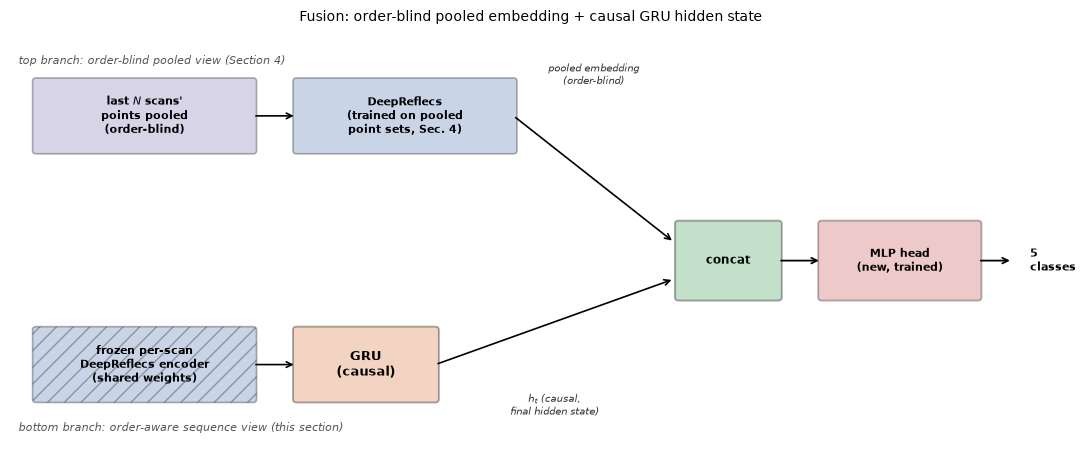
\includegraphics[width=0.85\textwidth]{results/final_report/final_report_30_0.png}
  \caption{Fusion: order-blind pooled embedding concatenated with the causal GRU's hidden state, both branches frozen.}
  \label{fig:fusion}
\end{figure*}

\begin{table*}[t]
  \centering
  \caption{GRU vs.\ Fusion Test Metrics}
  \label{tab:gru-fusion}
  \begin{tabular}{lrrrrrrr}
    \toprule
    & & \multicolumn{3}{c}{GRU alone} & \multicolumn{3}{c}{Fusion (pooled + GRU)} \\
    \cmidrule{3-5} \cmidrule{6-8}
    Class & Support & Precision & Recall & F1 & Precision & Recall & F1 \\
    \midrule
    car               & 76{,}572 & 0.952 & 0.935 & 0.944 & 0.953 & 0.933 & 0.943 \\
    large\_vehicle    & 15{,}555 & 0.817 & 0.841 & 0.829 & 0.810 & 0.845 & 0.827 \\
    two\_wheeler      & 11{,}466 & 0.844 & 0.909 & 0.875 & 0.849 & 0.906 & 0.877 \\
    pedestrian        & 35{,}091 & 0.895 & 0.905 & 0.900 & 0.888 & 0.914 & 0.901 \\
    pedestrian\_group & 40{,}081 & 0.904 & 0.895 & 0.900 & 0.910 & 0.890 & 0.900 \\
    \midrule
    \multicolumn{2}{l}{\textbf{Macro F1}} & \multicolumn{3}{l}{\textbf{0.8895}} & \multicolumn{3}{l}{\textbf{0.8897}} \\
    \bottomrule
  \end{tabular}
\end{table*}

\textbf{GRU alone: macro F1 = 0.8895} (+0.0260 over the pooling baseline).
\textbf{Fusion: macro F1 = 0.8897} (+0.0002 over GRU alone, within this
branch's own noise band for a single split, not a real additional gain)
(Table~\ref{tab:gru-fusion}).

The fusion model's confusion matrix shows two dominant error axes:
\emph{large\_vehicle} $\to$ \emph{car} at 15\% (the reverse direction is only
3.8\%), and \emph{pedestrian} $\leftrightarrow$ \emph{pedestrian\_group}
confuse each other both ways (6.6\% and 8.6\%). \emph{car} is the class
every \emph{large\_vehicle} error falls into, and the pedestrian/group
confusion is symmetric, not a one-directional bias (Fig.~\ref{fig:cm-fusion}).

\begin{figure}[t]
  \centering
  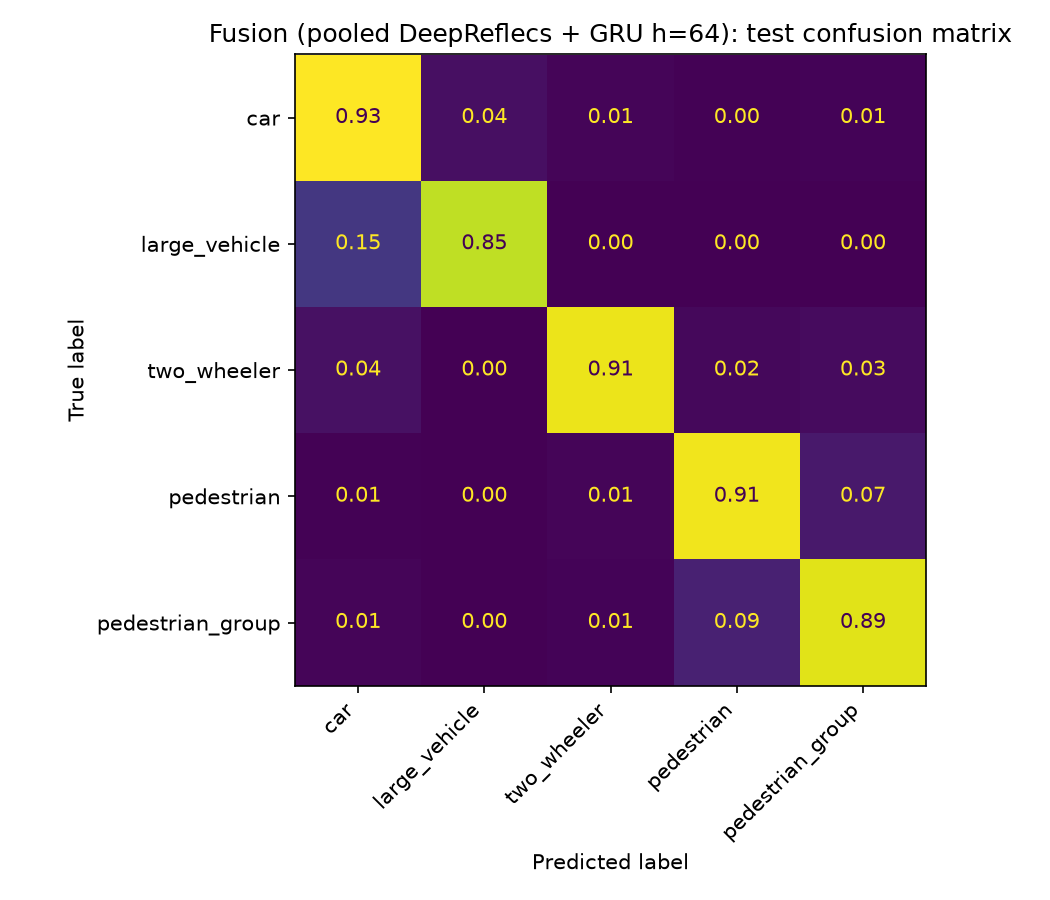
\includegraphics[width=0.85\columnwidth]{results/final_report/final_report_32_1.png}
  \caption{Fusion model ($N=20$, all sensors) confusion matrix, row-normalized.}
  \label{fig:cm-fusion}
\end{figure}

\subsection{Streaming Cost: O(N) vs.\ O(1)}

Every diagram and result above talks about a per-track FIFO buffer, but this
project never runs a live stream, scans arriving one at a time, hidden state
updated as they land. What is actually computed is an offline
reconstruction: each track's full scan history already exists in the
dataset, and the windowing functions just slice out, after the fact, what a
buffer \emph{would have held} at each point in time. The causal guarantee
still holds (a window never contains a future scan); it is just computed in
one pass over stored data rather than maintained incrementally.

This matters because the stateless GRU above is $O(N)$ per scan, not
$O(1)$. Every window replays its up-to-$N$ scans from a zeroed hidden state,
so a track running long enough needs a fresh $N$-step replay every single new
scan, not a cheap update -- a deployed version would redo almost the same
computation every step. That cost motivated testing a single-scan stateful
design instead: no window, one new scan fed per step, hidden state carried
from the previous step rather than reset to zero.
\[
h_0{=}0 \xrightarrow{\text{GRU}} h_1 \xrightarrow{\text{GRU}} h_2 \xrightarrow{\text{GRU}} h_3 \xrightarrow{\text{GRU}} h_4 \xrightarrow{\text{GRU}} h_5
\]
\[
\underset{(e_1)}{\phantom{h_1}} \qquad\ \underset{(e_2)}{\phantom{h_2}} \qquad\ \underset{(e_3)}{\phantom{h_3}} \qquad\ \underset{(e_4)}{\phantom{h_4}} \qquad\ \underset{(e_5)}{\phantom{h_5}}
\]

One continuous chain, $O(1)$ per scan, no replay. Naive training (gradients
detached and backpropagated after every single step) regressed hard, 0.8004
macro F1 against the stateless baseline's 0.8895. Letting gradients flow
across 20 consecutive steps before each detach (chunked truncated BPTT,
matching this branch's own $N=20$) recovered nearly all of it: 0.8846, within
this report's own ``under a point is a tie'' bar. So $O(1)$ streaming is
reachable without a real accuracy cost, but only if training lets the
model's gates see far enough back to learn it, not from the architecture
change alone.

For deployment, $O(1)$ is the better choice despite the slightly lower
score. trunc\_len=20 closes the gap to within this report's own noise band
(0.8846 vs.\ 0.8895), not a meaningful accuracy cost. The stateless design,
by contrast, has a real deployment cost that does not show up in macro F1 at
all: live, every track would need its full $N$-scan window replayed from a
zeroed hidden state at every new scan, on hardware the stateless offline
evaluation here never has to pay for. The $O(1)$ single-scan-stateful GRU is
a near-tie on accuracy with vastly cheaper per-scan inference, not the
stateless baseline that happens to be a hair ahead in this one offline
comparison.

$O(1)$ also changes the \emph{pedestrian}/\emph{pedestrian\_group} split,
which is mostly an instantaneous point-density judgment: one person's
cluster of points versus several overlapping ones. The stateless baseline
re-makes that judgment from $h_0{=}0$ every window; the $O(1)$ design
instead carries a hidden state across a track's full history, so once it
settles on ``this reads as one person'' early in a track, a later ambiguous
scan gets pulled toward that committed state instead of being judged fresh.
That explains pedestrian recall rising to 0.961 and pedestrian\_group recall
falling to 0.826 as the same mechanism from two sides.

This is not an unqualified improvement. A class judgment made early in a
track now propagates to every later scan instead of being re-evaluated each
window. Here the propagated judgment happened to be correct more often than
not, but the same mechanism would propagate an early misclassification just
as readily, nothing in the design distinguishes a correct lock-in from an
incorrect one. That is the practical argument for not carrying hidden state
unconditionally for a track's entire lifetime, and instead resetting it to
zero after a gap of no detections longer than some threshold
(gap\_threshold), the same mechanism discussed for track ID reuse. A reset
bounds how long a wrong early commitment can keep contaminating later
decisions, at the cost of losing carried state across real tracking gaps.

\section{Ablation Studies}

Everything below is single-split, not fold-validated: a proper 6-fold sweep
at this scale takes roughly a full day of compute per configuration, not run
here for every variant in Table~\ref{tab:ablation}.

\begin{table*}[t]
  \centering
  \caption{Ablation Studies}
  \label{tab:ablation}
  \footnotesize
  \begin{tabular}{p{0.26\textwidth}p{0.30\textwidth}p{0.36\textwidth}}
    \toprule
    What was tried & Result vs.\ its own reference & Reads as \\
    \midrule
    More GRU capacity ($h=128$) & Worse or flat vs.\ $h=64$ at every $N$/sensor scale tested & Not capacity-starved; more parameters overfit rather than help \\
    \addlinespace
    End-to-end fine-tuning (warmstart) of either the pooled encoder or the GRU's own per-scan encoder, at $N=20$ all-sensor & Both land \emph{below} their frozen baselines ($-0.0029$, $-0.0017$) & An already-good frozen encoder already sits near this task's ceiling; the one $N=10$ sensor2-only warmstart win does not generalize to this scale \\
    \addlinespace
    Post-hoc probability smoothing (causal, along a track) on the fusion model's output & Small positive: +0.0013 (moving average, $K=5$) to +0.0031 (IIR low-pass, same span) & Free accuracy at inference time, not a training-time fix \\
    \addlinespace
    Other sequence-mixing architectures (Transformer, a selective state-space model, point-level self-attention), same frozen per-scan embeddings & All land inside the same $\sim$0.86 to 0.89 macro F1 band as GRU/fusion & The bottleneck is upstream of which sequence-mixing mechanism is used, not solved by trying a different one \\
    \addlinespace
    Persistent GRU hidden state: warm-started from the previous stride=1 window's own $h_n$ instead of zero-initialized every window, $N=20$ all-sensor & $-0.0540$ vs.\ the plain (zero-init) GRU, the largest regression in this table & Helps nothing for stable-identity classes (\emph{car}, \emph{two\_wheeler} unaffected) and actively hurts \emph{pedestrian}/\emph{pedestrian\_group} ($-0.14$, $-0.12$ F1): those two are an instantaneous point-density judgment, not a persistent identity, and carried memory makes the model slower to update when that judgment should be re-made fresh every window \\
    \addlinespace
    Richer per-step input: each GRU timestep's embedding built from a sub\_n=5-scan pooled sub-window (its own encoder trained end-to-end on that pooled input) instead of a single scan, $N=20$ all-sensor & 0.8893, $-0.0002$ vs.\ the plain ($N=1$ per-step) GRU, flat per class too & The GRU's own 20-step recurrence over single-scan embeddings already recovers what a 5-scan pre-pooled embedding would add per step; pre-aggregating before the GRU is redundant with what its recurrence already extracts \\
    \addlinespace
    Wider embedding (point\_dim 32 to 128), same sparse input, tested both where it was never carried forward: the $N=20$ pooled baseline, and the GRU's own per-scan embeddings & Pooled: 0.8702, +0.0089 over the 0.8613 baseline. GRU: 0.8867, $-0.0028$ vs.\ the 0.8895 baseline & Wider capacity helps when there's a lot of raw information to represent (the $N=20$ pooled branch has hundreds of points); it does not help the GRU's input pipeline, where the bottleneck was never encoder capacity, the GRU's own 20-step integration already saturates whatever a per-scan embedding offers \\
    \bottomrule
  \end{tabular}
\end{table*}

All models/architectures (GRU, GRU $h=128$, Transformer $d=32$, Mamba,
point-level self-attention), all trained on the same frozen per-scan
embeddings, land within 0.86 to 0.89 macro F1 of each other, a 0.03 spread.
End-to-end fine-tuning of the encoder itself (warmstart) moved the number by
$-0.0017$ to $-0.0029$.

\section{Conclusions and Future Work}

Multi-scan accumulation improved the performance significantly: pooling
alone recovers most of the gap from the single-scan floor (0.7370
$\to$ 0.8613), and a causal GRU plus fusion recovers a further, smaller
amount ($\to$ 0.8897). Trying different designs for the sequence-mixing
stage, including its size, initialization, and mixing method, gives similar
results, suggesting there is limited room for further improvement in this
part of the model.

Concrete next steps, in order of expected information gained per hour spent:

\begin{enumerate}
\item \textbf{Fold-validate the current best configuration.} All results in
  this report come from a single split. Since differences of less than
  roughly one point may not be meaningful, this check is needed before
  treating small differences as real improvements.
\item \textbf{Compare errors across models.} Check which tracks are
  misclassified by the fusion model, GRU, and the other architectures. If
  the same tracks are consistently misclassified, the main limitation may
  come from the data or labels rather than the model.
\item \textbf{Inspect the confusion matrix manually.} Focus on cases such as
  \emph{large\_vehicle} predicted as \emph{car} and \emph{pedestrian} vs.\
  \emph{pedestrian\_group}. Compare these cases with the raw point clouds
  and RadarScenes ground truth, as these classes can be difficult to
  distinguish even for a human.
\item \textbf{Question the frozen per-scan embedding.} All sequence models
  use the same frozen DeepReflecs encoder for each scan. If this encoder is
  the main bottleneck, improving the sequence model is unlikely to lead to
  large gains.
\item \textbf{Fairly re-test the learned tracker-feature encoder.} A
  gradient-boosted-tree check (Section~IV-D) found real joint separability
  across the 8 patent-inspired features (AUC 0.78--0.92) that no single
  feature showed alone, motivating a temporal-fusion GRU built on that
  basis: a small trainable encoder over the raw per-scan tracker signal,
  fused with the frozen point embedding and trained end-to-end. It reached
  0.8938 macro F1, ahead of fusion's 0.8897, but using best-val-accuracy
  checkpoint restoration, a different training convention from every other
  result in this report (Appendix), so the comparison is not
  apples-to-apples as it stands. Fold-validating both under matching
  conventions, before treating this as a real gain, is the direct next
  step.
\end{enumerate}

\appendices
\section{Training Parameters}

Baseline: Fusion, pooled DeepReflecs + GRU $h=64$.

The fusion model combines two independently trained branches. The first
branch uses the $N=20$ pooled DeepReflecs encoder from Section~IV. The
second branch uses a separately trained $N=1$ DeepReflecs encoder, which
produces one embedding per scan. These embeddings are computed and stored
before training the GRU, so they are not recomputed for each window. The GRU
is then trained on the sequence of frozen embeddings.

The model is trained in four separate stages, with no joint training between
them. First, the $N=1$ DeepReflecs encoder is trained. The $N=20$ pooled
encoder is trained separately. A one-layer GRU with a hidden size of 64 is
then trained using the frozen $N=1$ embeddings. Finally, a small MLP fusion
head with two hidden layers and a hidden size of 16 is trained using the
concatenation of the pooled encoder output and the GRU's final hidden state.
During this final stage, only the fusion head is trained, while both
encoders and the GRU remain frozen.

All four stages use the same training setup: Adam with a learning rate of
$4\times10^{-5}$, a batch size of 128, and 100 epochs. The same
class-weighted cross-entropy loss is used, with class weights defined as
$\max(\text{count})/\text{count}_i$. No early stopping or checkpoint
restoration is used, so the weights from the final epoch are used.

The train/val/test split is fixed and done by \texttt{sequence\_name}, not by
scan; splitting by scan would leak information across splits. It uses
\texttt{StratifiedGroupKFold} with a 70/15/15 ratio, test carved out first,
then val from the remainder, and this same split is used for every result in
this report. Earlier, smaller-scale results in the project were instead
validated across 6 different sequence-grouped folds, to measure a
fold-to-fold noise band before trusting a gain as real.

\begin{thebibliography}{4}

\bibitem{schumann2021radarscenes}
O.~Schumann et al., ``RadarScenes: A Real-World Radar Point Cloud Data Set
for Automotive Applications,'' \emph{arXiv:2104.02493}, 2021.

\bibitem{ulrich2021deepreflecs}
M.~Ulrich, C.~Glaser, and F.~Timm, ``DeepReflecs: Deep Learning for
Automotive Object Classification with Radar Reflections,'' in \emph{IEEE
RadarConf}, 2021, arXiv:2010.09273.

\bibitem{ronneberger2015unet}
O.~Ronneberger, P.~Fischer, and T.~Brox, ``U-Net: Convolutional Networks for
Biomedical Image Segmentation,'' in \emph{MICCAI}, 2015.

\bibitem{aptiv2024patent}
Aptiv, ``Method for Classifying a Tracked Object,'' U.S.\ Patent
12{,}013{,}919~B2.

\end{thebibliography}

\end{document}
